\subsection{Fase 3: Limpieza y pre-procesamiento de datos}
En esta etapa se realizó la limpieza y el pre-procesamiento de los datos de destino para completarlos y hacerlos consistentes sin ningún tipo de ruido. Como se puede ver en la figura \ref{missing_data} la homogeneidad del conjunto de datos utilizado no generó valores perdidos, esto se debe a que fueron estandarizados por la secretaria de salud de la alcaldía municipal de Pereira.

\begin{figure}[h!]
	\centering
	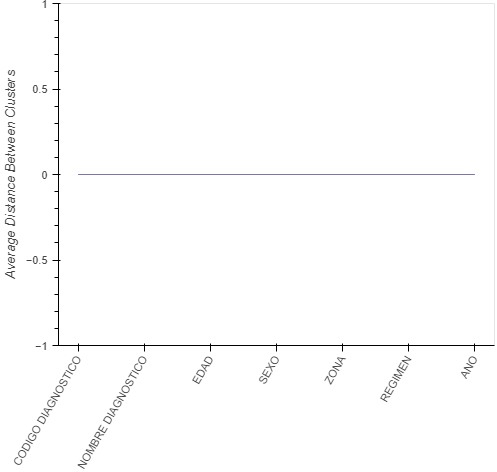
\includegraphics[width=0.9
	\linewidth]{IMAGENES/MISSING_DATA}
	\caption{Valores faltantes en el conjunto de datos.}
	\label{missing_data}
\end{figure} 


